%-------------------------------------------------------------------------------
%	DIRC TECHNOLOGY CHAPTER
%-------------------------------------------------------------------------------
\label{ch:dirc}
DIRC detectors are based on the concept of the Detection of Internally Reflected Cherenkov light (DIRC) produced in a solid radiator bar to identify charged particle. It is a special type of Cherenkov counter, which uses the unique properties of Cherenkov radiation to identify charged particle species.

%-------------------------------------------------------------------------------
%	CHERENKOV RADIATION SECTION
%-------------------------------------------------------------------------------
\section{Cherenkov Radiation}
Einstein postulated in his Theory of Relativity that the speed of light in a vacuum, $c$, is the limit of the velocity of massive particles. In an optically transparent medium, however, the speed at which light propagates is modified: $c_{med} = c/n$, where $n$ is the index of refraction of the medium. Pavel Cherenkov discovered in 1934 that massive particles moving through a medium faster than the speed of light in that medium emit light in the form of now-called Cherenkov radiation. Cherenkov was able to establish several interesting properties of this radiation: it is only emitted from charged particles above a certain velocity threshold $v > c/n$, the intensity is proportional to the particle's path length, emission is prompt, and the light is polarized with a continuous wavelength spectrum. Later in 1937 Ilya Frank and Igor Tamm theoretically formulated this radiation with fantastic agreement to Cherenkov's findings, and the three shared the 1958 Nobel Prize in Physics for their efforts \cite{CherenkovHistory}.

Further studies confirmed that Cherenkov radiation is emitted uniformly in azimuth ($\phi_c$) around the particle's direction of travel with the polar opening angle $\thetaC$ defined as

\begin{equation}
	\cos\thetaC = \frac{1}{\beta n(\lambda)},
	\label{eq:cherenkovformula}
\end{equation}

where $\beta = v_p/c$, $v_p$ is the particle's velocity, and the index of refraction is a function of the emitted photon wavelength. In a normal, dispersive optical medium the opening half-angle of the shock wave produced by the Cherenkov radiation, $\eta_C$ defined in Figure \ref{fig:cherenkovcone}, is not complementary to the Cherenkov angle. The relationship between the two is given by

\begin{equation}
	\cot\eta_C = \left[\frac{\diff}{\diff\omega}(\omega \tan\thetaC) \right]_{\omega_0} = \left[\tan\thetaC + \beta^2\omega n(\omega) \frac{\diff n}{\diff\omega}\cot\thetaC \right]_{\omega_0}
	\label{eq:openingangle}
\end{equation}

where $\omega_0$ is the central vale of the considered frequency range. Because the second term in (\ref{eq:openingangle}) is zero only for non-dispersive media the shock wave front is not perpendicular to the Cherenkov cone in real detectors.

\begin{figure}[ht]
	\centering
	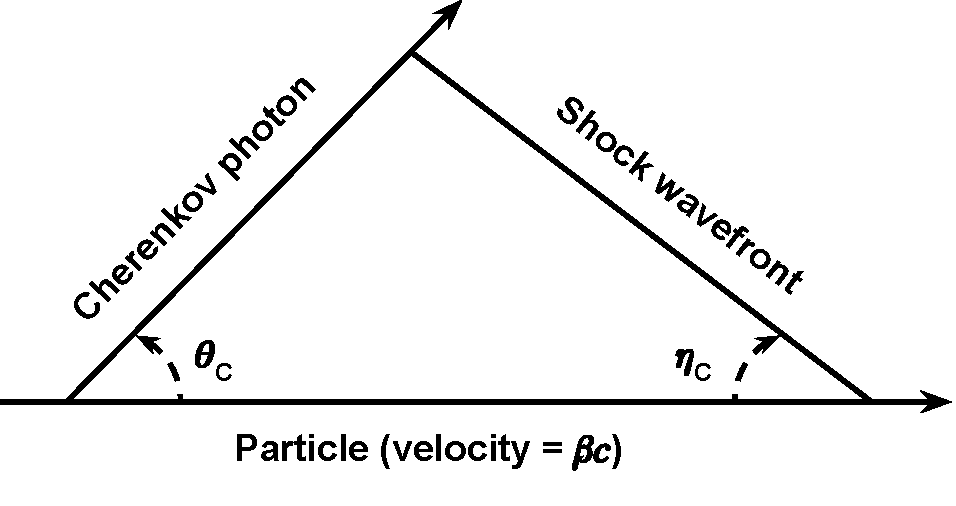
\includegraphics[scale=1]{Cherenkov_cone.pdf}
	\caption{Illustration of the Cherenkov cone.}
	\label{fig:cherenkovcone}
\end{figure}

Because particles lose very little energy when radiating Cherenkov photons the emission is very weak. The number of photons $N_{photons}$ emitted per path length $L$ (in cm) by a moving particle with charge $z$ is given by the Frank-Tamm equation

\begin{equation}
	\frac{N_{photons}}{L} = \frac{\alpha^2 z^2}{r_e m_e c^2} \int \sin^2\thetaC (E) \diff E
	\label{eq:nphotons}
\end{equation}
where E is the photon energy in eV, the integral is taken over the region where $n(E)$ is greater than 1, and $\frac{\alpha^2 z^2}{r_e m_e c^2} = 370\unit{cm}^{-1}\unit{eV}^{-1}$.

%-------------------------------------------------------------------------------
%	APPLYING TO PID SECTION
%-------------------------------------------------------------------------------
\section{Applying the Cherenkov Effect to Particle ID}
In order to identify particle species one must know both the mass and charge of the particle in question. Because the Cherenkov angle encodes the particle's velocity it is, in principle, a simple matter to measure the particle's momentum with a tracking chamber as well as the velocity obtained from (\ref{eq:cherenkovformula}) to determine the mass and charge. Figure \ref{fig:angleseperation} shows how different particle species can be distinguished for a given momentum in fused silica.

Threshold Cherenkov counters are detectors used for particle identification (PID) by exploiting the fact that only particles above the threshold velocity $\beta > 1/n$ will emit Cherenkov photons. The information about a particle's velocity can be combined with momentum information from a tracking system to determine the mass as \cite{ParticleDetectionHandbook}

\begin{equation}
	m = \frac{p}{c} \sqrt{n^2 \cos^2\thetaC - 1}
	\label{eq:mass}
\end{equation}

\begin{figure}[ht]
	\centering
	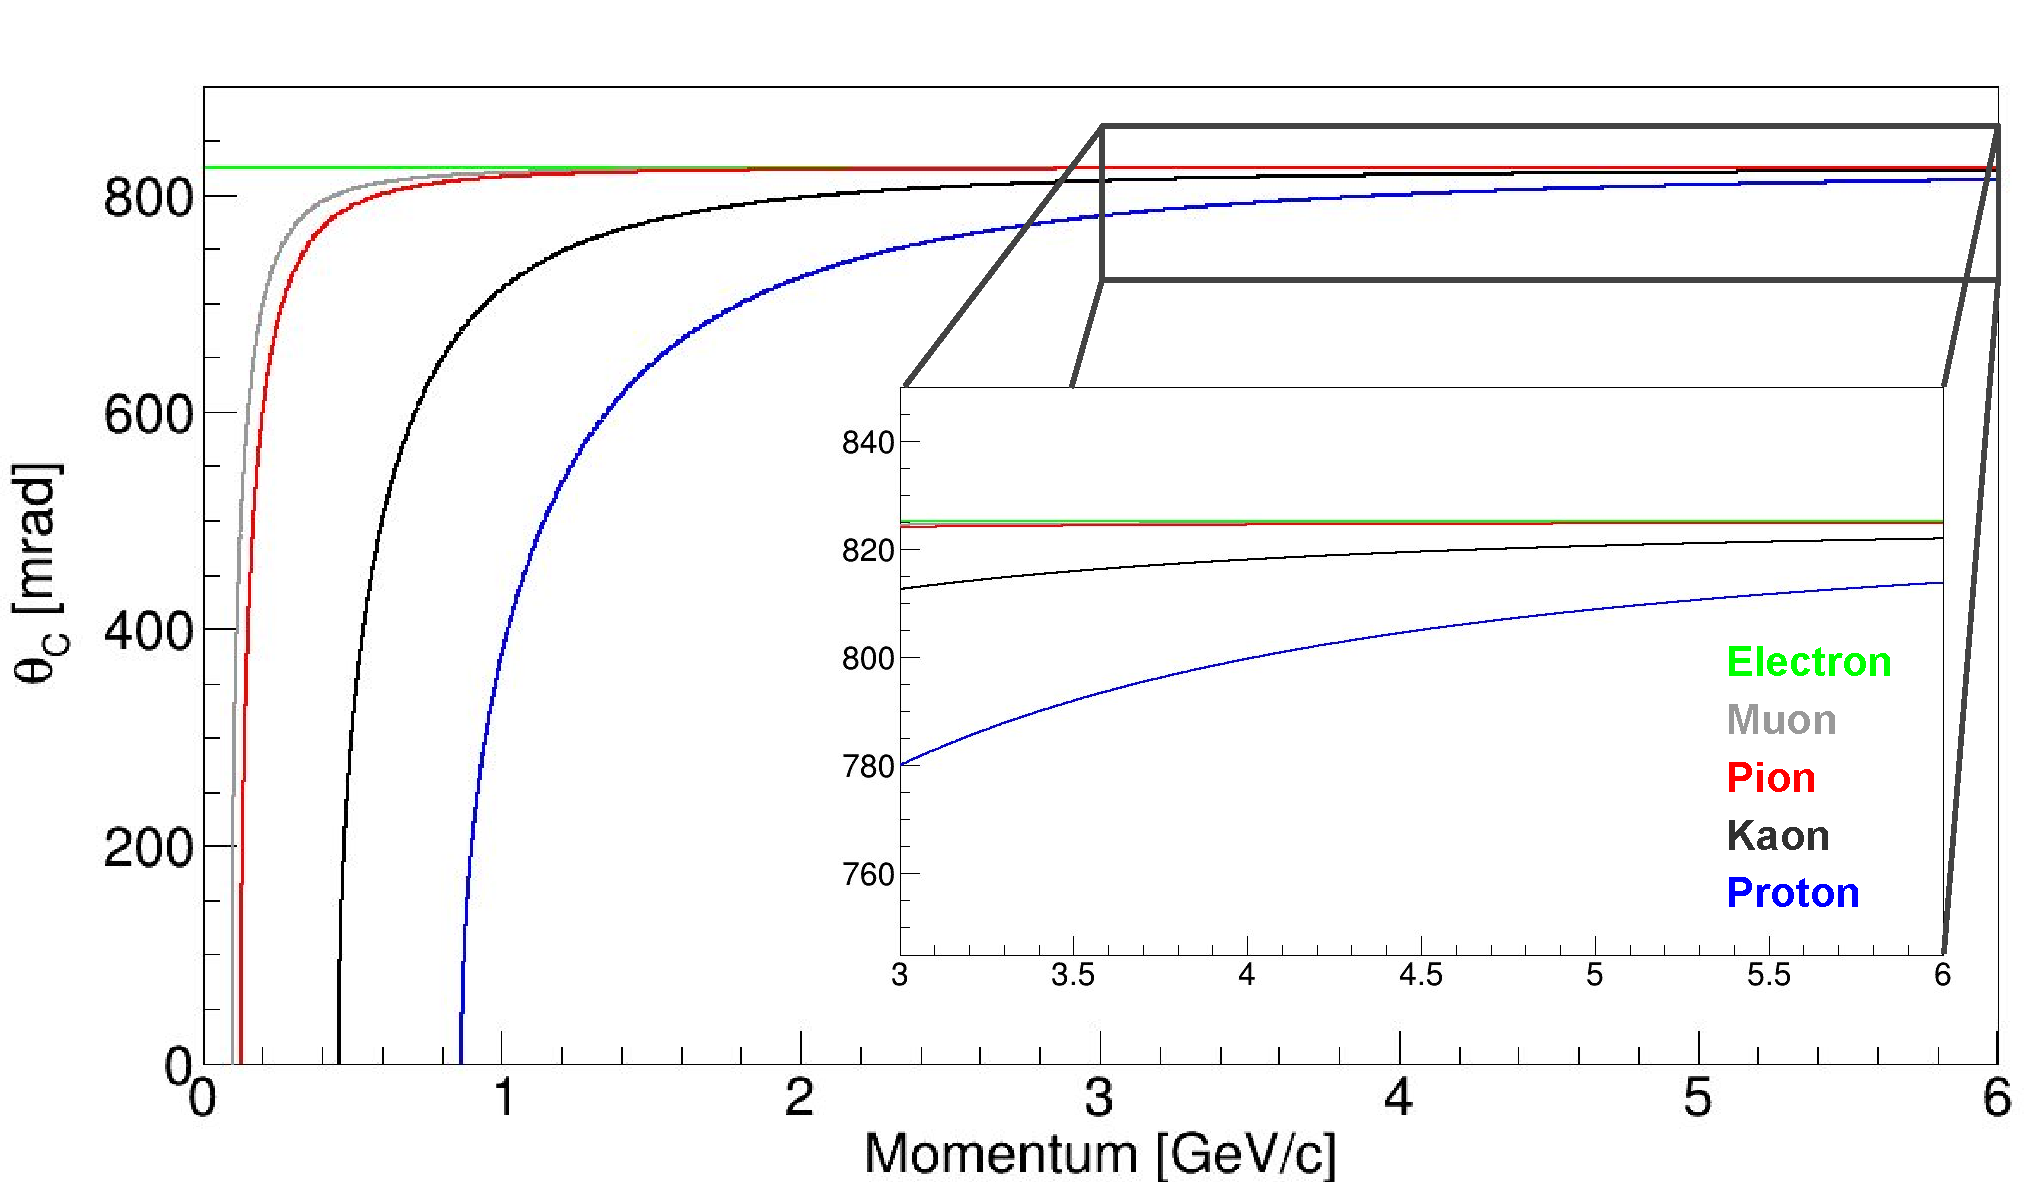
\includegraphics[width=\textwidth]{angle_seperation_enhance.pdf}
	\caption{Particle momentum [GeV/c] versus Cherenkov angle [mrad] for different particle species in fused silica ($n \approx 1.473$). The zoomed image shows that it is indeed possible to differentiate pions, kaons, and protons at higher particle momenta.}
	\label{fig:angleseperation}
\end{figure}

%-------------------------------------------------------------------------------
%	RICH SECTION
%-------------------------------------------------------------------------------
\section{Ring Imaging Detectors}
Ring Imaging Cherenkov (RICH) detectors are designed to efficiently identify and separate different particle species over a wide range of momenta. A basic RICH system is shown in Figure \ref{fig:rich_basics}. 

\begin{figure}[ht]
	\centering
	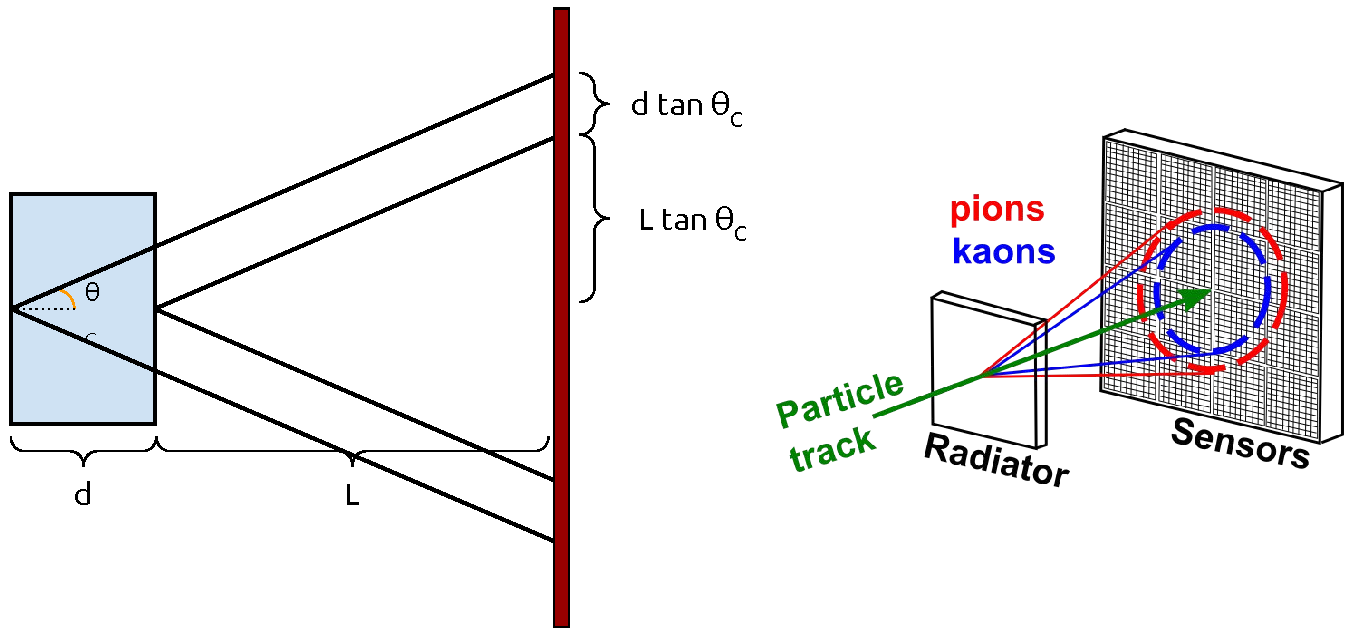
\includegraphics[width=\textwidth]{RICH_rings.pdf}
	\caption{Basic concept of a proximity focusing Ring Imaging Cherenkov (RICH) detector (a), and an example of how they can be used to do PID based on particle mass (b).}
	\label{fig:rich_basics}
\end{figure}

A volume of radiator, either gaseous (e.g. $C_{4}F_{10}$) or solid (e.g. aerogel), is positioned upstream of an array of photosensors. A charged particle traveling through a thin radiator above the threshold velocity will continuously emit Cherenkov photons in a cone. The resulting image on the photosensor array is an annulus of thickness $d\tan\thetaC$ and an inner radius of $L\tan\thetaC$, where $d$ is the distance the particle traveled inside the radiator, $L$ is the distance between the radiator and the photsensors, and  $\thetaC$ is the usual Cherenkov angle (Figure \ref{fig:rich_basics}b). PID is done by measuring the average radius of the annulus and reconstructing the Cherenkov angle geometrically.


%-------------------------------------------------------------------------------
%	DIRC SECTION
%-------------------------------------------------------------------------------
\section{DIRC Detectors}
DIRC detectors work much the same way as a RICH in that collect Cherenkov photons produced from a radiating material and use the created image on the photosensors to reconstruct the Cherenkov angle. In the case of a DIRC, the radiating medium is also used as a light guide as some of the Cherenkov photons undergo total internal reflection inside the radiator and are guided towards one end of the radiator to a readout (Figure \ref{fig:dircbasics}). The radiator of choice is a solid bar made of fused silica, with an index of refraction $n \approx 1.473$. A rectangular cross section and highly smoothed and polished sides ensure that the magnitude of the Cherenkov angle is preserved during internal reflection. Photons that are created propagating away from the readout are reflected back towards the readout by a mirror. Once the photons exit the radiator they are allowed to separate through an expansion volume before being imaged in both ($x, y$) position as well as time. The arrival position and propagation time of each detected photon are combined with tracking information to reconstruct the Cherenkov angle and determine the corresponding PID likelihoods.

\begin{figure}[ht]
	\centering
	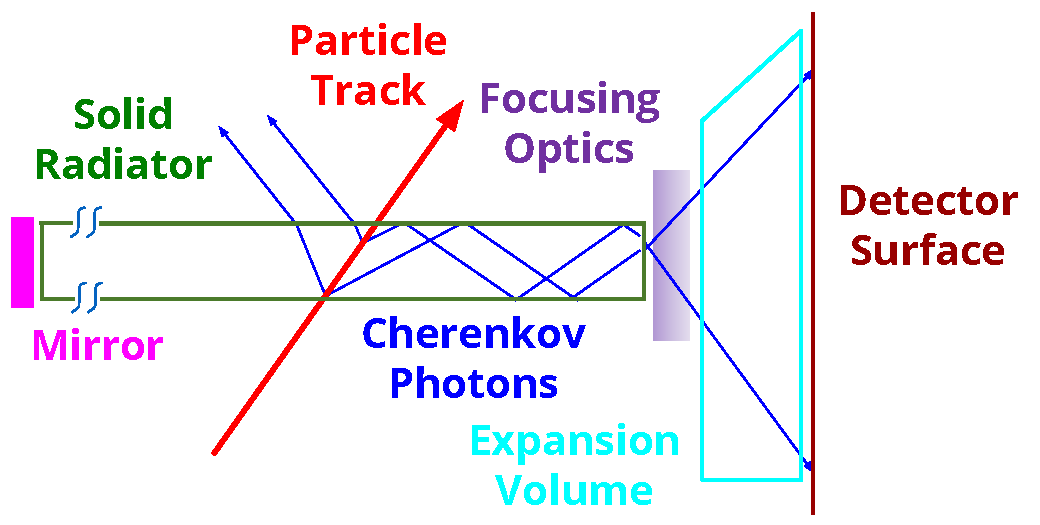
\includegraphics[scale=0.7]{DIRC_components.pdf}
	\caption{The basic components of a DIRC detector: a solid radiator, typically fused silica (green); a mirror to redirect backward-going photons (pink); optional focusing optics (purple); an expansion volume to allow photons to separate in space (cyan); and a detector surface to record the position and arrival time of Cherenkov photons (maroon).}
	\label{fig:dircbasics}
\end{figure}

The performance of a DIRC detector is given by the resolution in the Cherenkov polar opening angle of the particle track, $\sigma_{\thetaC,\text{track}}^2$, which can be written as:

\begin{equation}
	\sigma_{\thetaC,\text{track}}^2 = \sigma_{\thetaC}^2 / N_{\gamma} + \sigma_{\text{correlated}}^2
	\label{eq:performance}
\end{equation}

where $\sigma_{\thetaC}$ is the average single photon Cherenkov angle resolution, $N_{\gamma}$ is the number of measured photons per track, and $\sigma_{\text{correlated}}$ includes several correlated terms that contribute to the resolution such as the uncertainty in the particle track direction coming from external tracking systems. Because the track direction is crucial to the reconstruction of the Cherenkov angle, this error needs to be small for the performance to not suffer. For the EIC a tracking resolution on the order of 1 mrad is required for adequate PID.

\begin{figure}[ht]
	\centering
	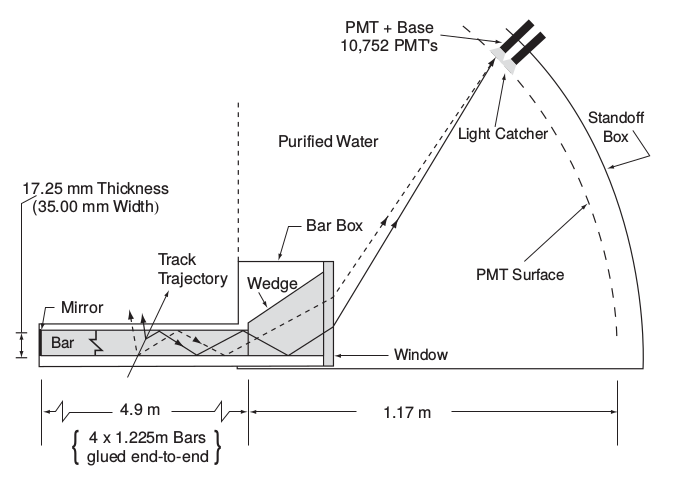
\includegraphics[width=\textwidth]{BaBar_DIRC.png}
	\caption{Schematic of BaBar DIRC and imaging region.}
	\label{fig:babardirc}
\end{figure}

As of the writing of this thesis the only DIRC detector used in a full experiment is the BaBar DIRC at SLAC National Accelerator Laboratory, which was successfully operated from 1999 through 2008 \cite{BaBarDIRC}. It proved to be a robust, stable, and easy to operate system for more than 8 years, providing excellent pion/kaon separation for all tracks from $B$-meson decays. It used 4.9 m long radiator bars with a rectangular cross section of $17.25 \times 35 \unit{mm}^2$. Each bar was made of four $1.225\unit{m}$ long fused silica bars glued end-to-end. The bars were placed in 12 hermetically sealed containers, called bar boxes, each holding 12 radiator bars for a total of 144 bars. At the end of each box was attached a wedge of fused silica and a window to allow the photons to expand before entering the water-filled expansion volume and being read out on one of 10,752 photomultiplier tubes (see Figure \ref{fig:babardirc}). Figure \ref{fig:babarperformance} summarizes the performance of the BaBar DIRC, showing excellent Cherenkov angle reconstruction (2.5 mrad, only 14\% larger than the design goal of 2.2 mrad) and photon yield per track.

\begin{figure}[ht]
	\centering
	a)%
	\raisebox{-1.0\height}{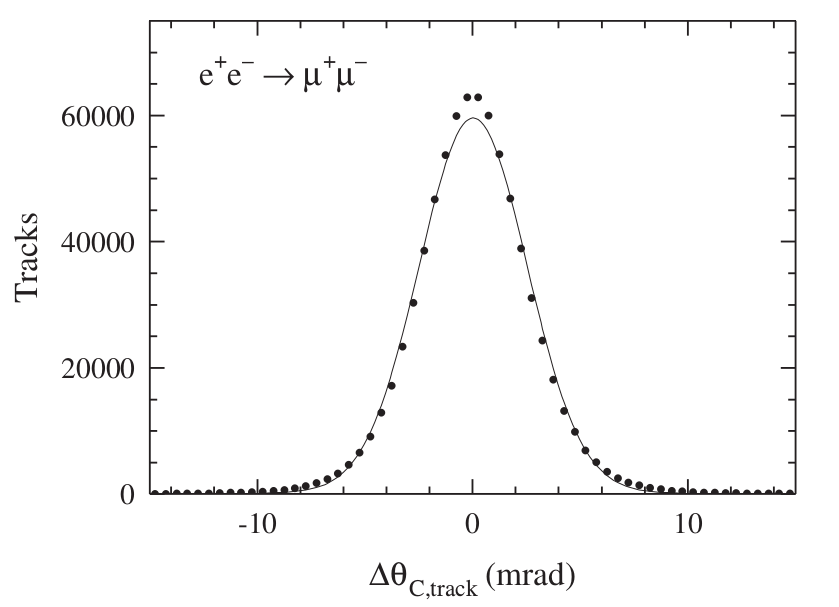
\includegraphics[width=0.5\textwidth]{BaBar_SPR.png}}%
	b)%
	\raisebox{-1.0\height}{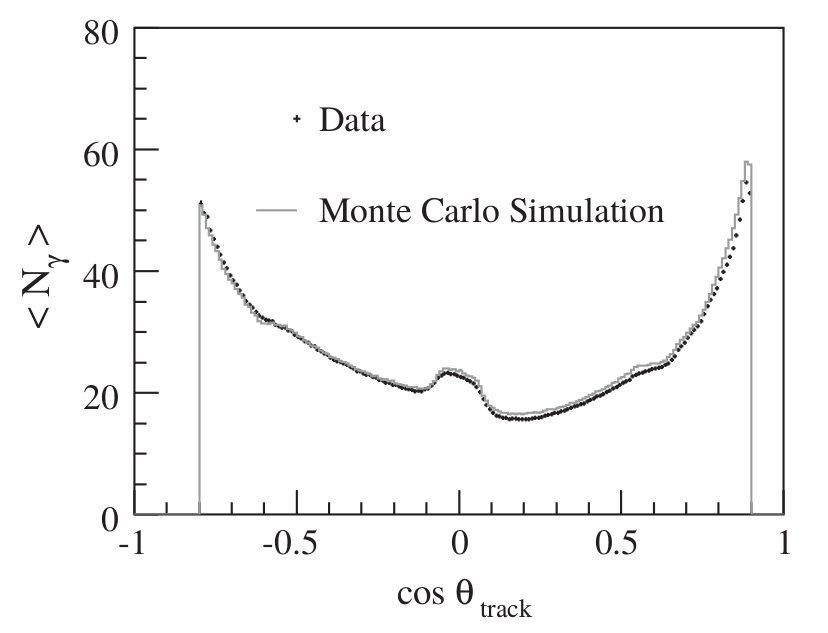
\includegraphics[width=0.5\textwidth]{BaBar_NPH.png}}
	\caption{Performance of the BaBar DIRC for $e^{+}e^{-} \rightarrow \mu^{+}\mu^{-}$ events. a) shows the difference between the measured and expected Cherenkov angle (dots) and a Gaussian fit to the data with a 2.5 mrad width (line). b) is the average number of detected photons vs. track polar angle for data (dots) and Geant4 simulation (line).}
	\label{fig:babarperformance}
\end{figure}

\subsection{Evolution of DIRC Detector Designs}
\subsection{DIRCs in Future Experiments}
The BaBar DIRC has since inspired many other experiments to utilize this new, novel PID system in a variety of ways (Figure \ref{fig:dirc_evolution}. The Focusing DIRC (FDIRC) proposed for the now-cancelled SuperB collider in Italy was the first to propose using some form of focusing for the Cherenkov photons, allowing for a factor of 10 smaller expansion volume \cite{FDIRC}. The barrel DIRC for the PANDA experiment at FAIR in Germany will use shorter radiator bars for a more compact design, while the PANDA disc-shaped DIRC will be used in the 
Along with the EIC, there are several detectors currently being planned that will include the use of DIRC detectors of some variation for their PID needs, including: the PANDA experiment at FAIR in Germany, the Belle II detector at the KEKB accelerator in Japan, the ToRCH detector at LHCb in France, and the GlueX experiment at JLab in the U.S.
\comment{WRITE A SHORT PARAGRAPH ABOUT EACH OF THE ABOVE EXPERIMENTS AND GIVE A CITATION FOR EACH}

\begin{figure}
	\centering
	%\includegraphics[scale=1]{DIRC_evolution.pdf}
	\caption{Evolution of the DIRC concept. From top left to bottom right:}
	\label{fig:dirc_evolution}
\end{figure}
